\begin{frame}
  \frametitle{\textbf{Jets in Experiment}}
  \begin{columns}
    \column{0.5\textwidth}
    \begin{itemize}
    \item A jet is the result of a \textbf{jet algorithm}, which is a computational process to cluster groups of collimated particles
    \item There are many types of jet algorithms, often differentiated by their choice of ``distance parameter''
    \end{itemize}
    \begin{align*}
      d_{ij} &= \min(p_{\text{T},i}^{2k},p_{\text{T},j}^{2k} )\cfrac{\Delta R_{ij}^2}{R^2} \\
      &k = 0 \to \text{Cambridge-Aachen algorithm} \\
        &k = 1 \to k_{\text{T}} \text{ algorithm} \\
          &k = -1 \to \text{anti-}k_{\text{T}} \text{ algorithm} \\
    \end{align*}
    \begin{itemize}
    \item Iteratively cluster pairs of tracks with smallest $d_{ij}$ and ``build'' jets
    \end{itemize}

    \column{0.5\textwidth}
    \centering
    \begin{tikzpicture}
      \node{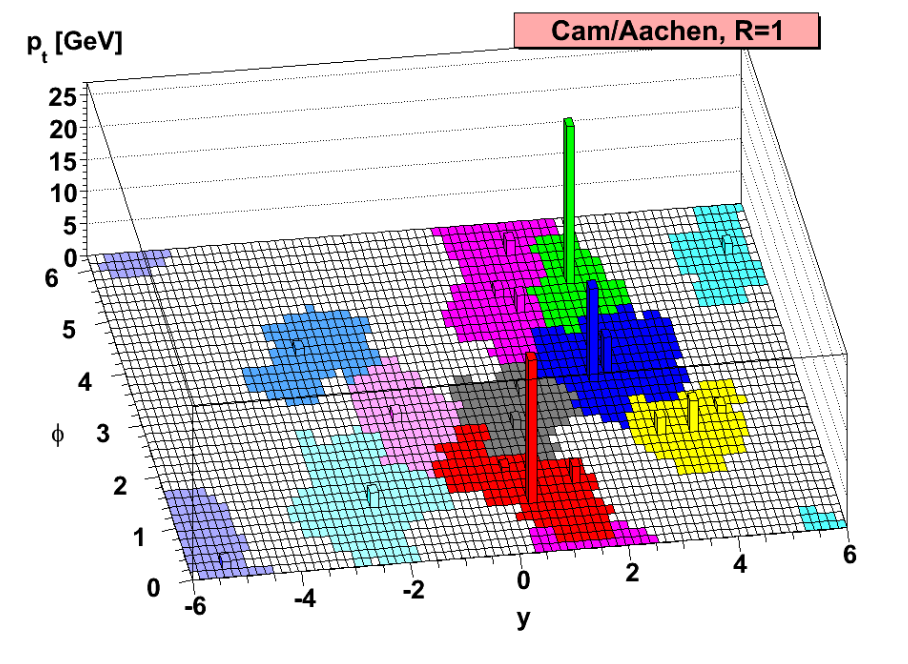
\includegraphics[width=0.6\textwidth]{cam-aachen.png}};
    \end{tikzpicture}

    \centering
    \begin{tikzpicture}
      \node{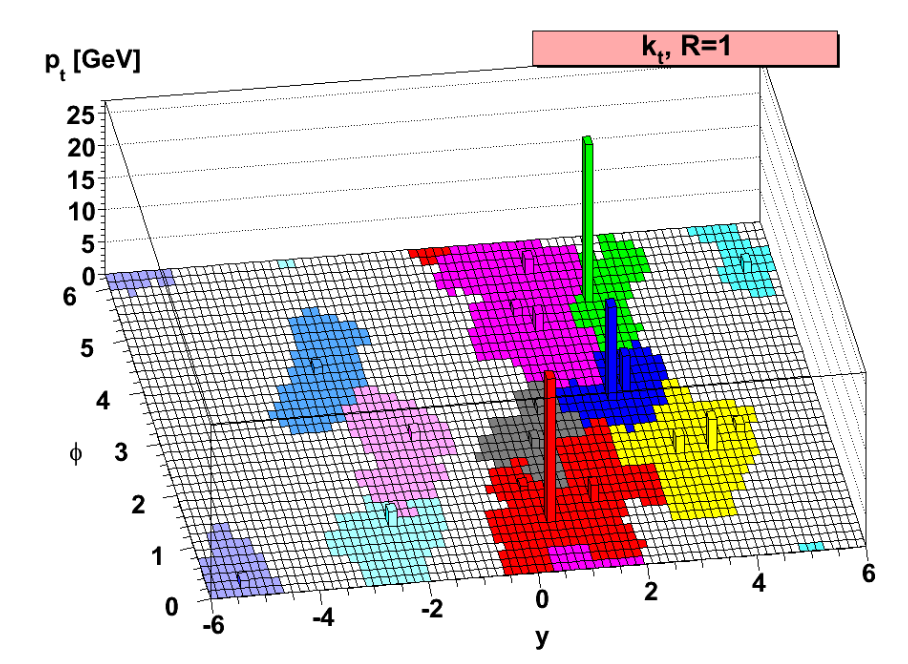
\includegraphics[width=0.6\textwidth]{kt.png}};
    \end{tikzpicture}

    \centering
    \begin{tikzpicture}
      \node{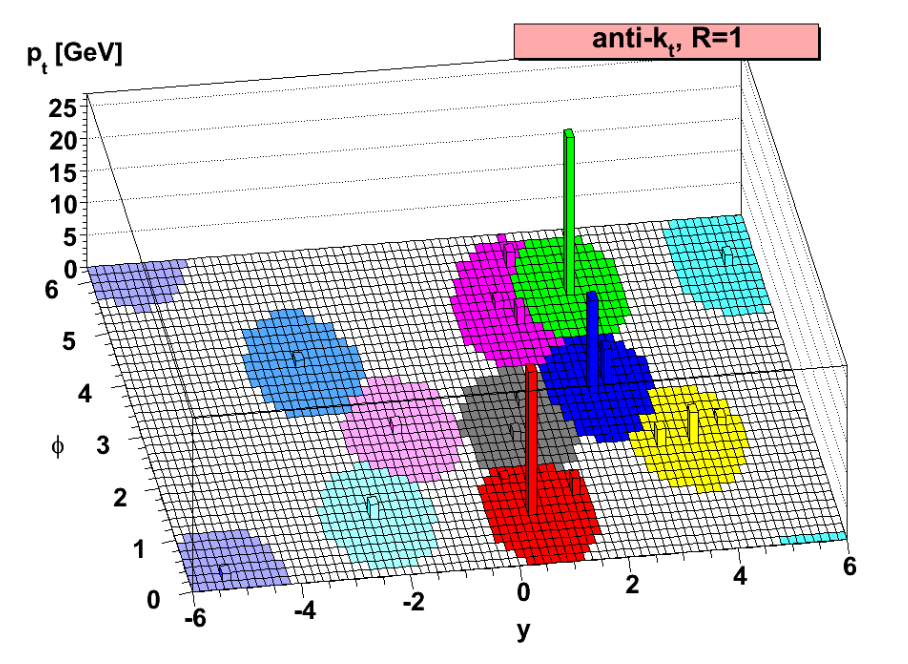
\includegraphics[width=0.6\textwidth]{anti-kt.png}};
    \end{tikzpicture}
  \end{columns}
\end{frame}
